\graphicspath{{./tenth/img}}

\section*{\LARGE{Введение}}
\addcontentsline{toc}{section}{Введение}

\textbf{Задание}:
\begin{itemize}
	\item Реализовать пример с применением технологий стилей;
	\item Реализовать пример с применением технологий тем;
	\item Реализовать пример создания собственной темы;
	\item Реализовать пример с применением темы к activity;
	\item Реализовать пример с применением темы к иерархии виджетов;
	\item Реализовать пример с применением определения меню в xml;
	\item Реализовать пример с наполнением меню элементами;
	\item Реализовать обработку нажатий в меню;
	\item Реализовать программное создание меню;
	\item Реализовать программное создание подменю.;
	\item Реализовать группы в меню;
	\item Реализовать программное создание групп в меню и подменю.
\end{itemize}

\clearpage

\section*{\LARGE{Выполнение практической работы}}
\addcontentsline{toc}{section}{Выполнение практической работы}

\section{Стили и темы}
\subsection{Стили}
Мы можем настроить элемент с помощью различных атрибутов, которые
задают высоту, ширину, цвет фона, текста и так далее. Но если у нас
несколько элементов используют одни и те же настройки, то мы можем
объединить эти настройки в стили.\par
Все эти TextView имеют одинаковый набор свойств, и, к примеру, если нам
захочется изменить цвет текста, то придется менять его у всех трех TextView.
Данный подход не оптимален, а более оптимальный подход представляет
использование стилей, которые определяются в проекте в папке res/values.
Итак, добавим в проект в папку res/values новый элемент Value Resourse
File, который назовем styles.xml (Листнинг~\ref{lst:xml:style}).

\begin{lstlisting}[language=XML
	, label=lst:xml:style
	]
<?xml version="1.0" encoding="utf-8"?>
<resources>
    <style name="FirstStyle">
        <item name="android:layout_width">0dp</item>
        <item name="android:layout_height">wrap_content</item>
        <item name="android:textColor">#3f51b5</item>
        <item name="android:textSize">28sp</item>
        <item name="android:gravity">center</item>
    </style>
</resources>
\end{lstlisting}

Здесь определен новый стиль TextViewStyle, который с помощью элементов
item задает значения для атрибутов TextView.\par
Стиль задается с помощью элемента <style>. Атрибут name указывает на
название стиля, через которое потом можно ссылаться на него.
Необязательный атрибут parent устанавливает для данного стиля
родительский стиль, от которого дочерний стиль будет наследовать все свои
характеристики.\par
С помощью элементов item устанавливаются конкретные свойства виджета,
который принимает в качестве значения атрибута name имя
устанавливаемого свойства.\par
Теперь применим стиль, изменим файл разметки, как показано
в листинге~\ref{lst:xml:style:use}.

\begin{lstlisting}[language=XML
	, label=lst:xml:style:use
	]
<?xml version="1.0" encoding="utf-8"?>
<androidx.constraintlayout.widget.ConstraintLayout xmlns:android="http://schemas.android.com/apk/res/android"
    xmlns:app="http://schemas.android.com/apk/res-auto"
    android:layout_width="match_parent"
    android:layout_height="match_parent"
    xmlns:tools="http://schemas.android.com/tools"
    tools:context=".MainActivity">
    <TextView
        android:id="@+id/textView1"
        android:layout_width="0dp"
        android:layout_height="wrap_content"
        style="@style/FirstStyle"
        android:text="Android Lollipop"
        app:layout_constraintLeft_toLeftOf="parent"
        app:layout_constraintRight_toRightOf="parent"
        app:layout_constraintTop_toTopOf="parent"
        app:layout_constraintBottom_toTopOf="@+id/textView2" />
    <TextView
        android:id="@+id/textView2"
        android:layout_width="0dp"
        android:layout_height="wrap_content"
        style="@style/FirstStyle"
        android:text="Android Marshmallow"
        app:layout_constraintLeft_toLeftOf="parent"
        app:layout_constraintRight_toRightOf="parent"
        app:layout_constraintBottom_toTopOf="@+id/textView3"
        app:layout_constraintTop_toBottomOf="@+id/textView1"
        />
    <TextView
        android:id="@+id/textView3"
        android:layout_width="0dp"
        android:layout_height="wrap_content"
        style="@style/FirstStyle"
        android:text="Android Nougat"
        app:layout_constraintLeft_toLeftOf="parent"
        app:layout_constraintRight_toRightOf="parent"
        app:layout_constraintBottom_toBottomOf="parent"
        app:layout_constraintTop_toBottomOf="@+id/textView2" />
</androidx.constraintlayout.widget.ConstraintLayout>
\end{lstlisting}

\subsection{Темы}
Кроме применение отдельных стилей к отдельным элементам, мы можем
задавать стили для всего приложения или activity в виде тем. Тема
предтавляет коллекцию атрибутов, которые применяются в целом ко всему
приложению, классу activity или иерархии виджетов.\par
Мы можем сами создать тему. Однако Android уже предоставляет несколько
предустановленных тем для стилизации приложения, например,
Theme.AppCompat.Light.DarkActionBar и ряд других.\par
По умолчанию приложение уже применяет темы. Так, откроем файл
AndroidManifest.xml. В нем мы можем увидеть следующее определение
элемента application, представляющего приложение
(листинг~\ref{lst:xml:manifest}).

\begin{lstlisting}[language=XML
	, label=lst:xml:manifest
	]
<application
        android:allowBackup="true"
        android:dataExtractionRules="@xml/data_extraction_rules"
        android:fullBackupContent="@xml/backup_rules"
        android:icon="@mipmap/ic_launcher"
        android:label="@string/app_name"
        android:roundIcon="@mipmap/ic_launcher_round"
        android:supportsRtl="true"
        android:theme="@style/Theme.Tenth"
        ...
\end{lstlisting}

Задание темы происходит с помощью атрибута android:theme. В данном
случае используется ресурс, который называется в моем случае
Theme.Tenth. По умолчанию файлы тем определены в папке res/values. В
частности, здесь можно найти условный каталог themes, в котором по
умолчанию есть два элемента themes.xml. Один файл представляет светлую тему,
а другой --- темную.\par
При необходимости мы можем изменить характеристики или дополнить
тему новыми стилевыми характеристиками. Например, изменим цвет
свойства colorPrimary, которое применяется в том числе в качестве фонового
цвета заголовка и кнопки (рис.~\ref{fig:theme}).

\begin{image}
	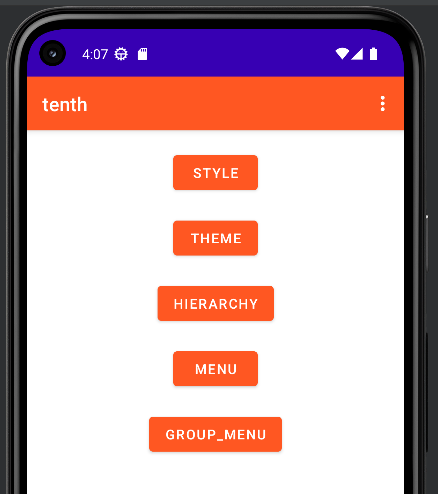
\includegraphics[width=0.4\textwidth]{Screenshot from 2023-04-27 16-08-05}
	\caption{Пример измененной темы}
	\label{fig:theme}
\end{image}

\subsection{Создание собственной темы}
Вместо использования встроенных тем мы можем создать свою. Для этого
добавим в папку res/values новый файл mythemes.xml и определим в нем
код, как показано в листинге~\ref{lst:xml:theme}

\begin{lstlisting}[language=XML
	, label=lst:xml:theme
	]
<?xml version="1.0" encoding="utf-8"?>
<resources>
    <style name="MyTheme" parent="Theme.AppCompat.Light">
        <item name="android:textColor">#FF018786</item>
        <item name="android:textSize">28sp</item>
    </style>
</resources>
\end{lstlisting}

Итак, мы создали стиль "MyTheme", который унаследован от стиля
Theme.AppCompat.Light. В этом стиле мы переопределили два свойства:
высоту шрифта (textSize) --- 28sp, а также цвет текста
(textColor) --- \#FF018786.\par
Теперь можно определить этот стиль в качестве темы приложения в файле
AndroidManifest.xml.\par
Результат проиллюстрирован на рисунке~\ref{fig:theme:use}

\begin{image}
	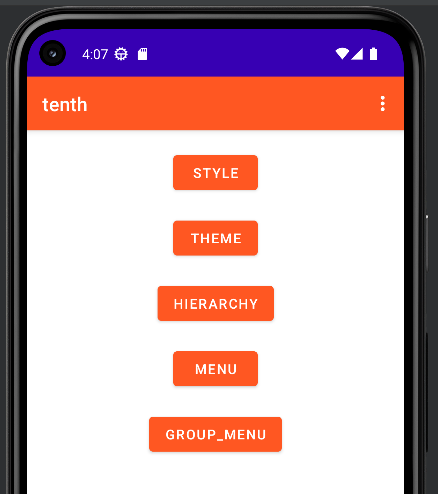
\includegraphics[width=0.4\textwidth]{Screenshot from 2023-04-27 16-08-05}
	\caption{Пример измененной темы}
	\label{fig:theme:use}
\end{image}

\subsection{Применение темы к activity}
Выше темы применялись глобально ко всему приложению. Но также можно
применить их к отдельному классу Activity. Для этого надо подкоррективать
файл манифеста AndroidManifest. Например, как показано в 
листинг~\ref{lst:xml:theme}.

\begin{lstlisting}[language=XML
	, label=lst:xml:theme
	]
<application
	android:allowBackup="true"
	android:dataExtractionRules="@xml/data_extraction_rules"
	android:fullBackupContent="@xml/backup_rules"
	android:icon="@mipmap/ic_launcher"
	android:label="@string/app_name"
	android:roundIcon="@mipmap/ic_launcher_round"
	android:supportsRtl="true"
	android:theme="@style/Theme.Tenth"
	tools:targetApi="31">
	<activity
		android:name=".Theme"
		android:exported="false"
		android:theme="@style/MyTheme">
		<meta-data
			android:name="android.app.lib_name"
			android:value="" />
	</activity>
\end{lstlisting}

Атрибут android:theme элемента <activity> указывает на применяемую к
MainActivity тему. То есть глобально к приложению применяется тема
"Theme.Tenth", а к Theme - "MyTheme".

\subsection{Применение темы к иерархии виджетов}
Также можно применить тему к иерархии виджетов, установив атрибут
android:theme у элемента, к которому (включая его вложенные элементы) 
мы хотим применить тему. Например, примение темы к ConstraintLayout и ее
элементам, показан в листинге~\ref{lst:xml:theme:hierarchy}.

\begin{lstlisting}[language=XML
	, label=lst:xml:theme:hierarchy
	]
<?xml version="1.0" encoding="utf-8"?>
<androidx.constraintlayout.widget.ConstraintLayout
    xmlns:android="http://schemas.android.com/apk/res/android"
    xmlns:app="http://schemas.android.com/apk/res-auto"
    xmlns:tools="http://schemas.android.com/tools"
    android:layout_width="match_parent"
    android:layout_height="match_parent"
    tools:context=".Hierarchy"

    android:theme="@style/MyTheme">

	...
\end{lstlisting}

\section{Меню}
\subsection{Определение меню в xml}
Меню, как и файлы интерфейса или изображений, также представляет собой
ресурс. Однако при создании нового проекта с Empty Activity по умолчанию
нет никаких ресурсов меню, поэтому при необходимости их нужно добавлять
вручную.\par
По умолчанию этот файл определяет один пустой элемент menu
(Листнинг~\ref{lst:xml:menu}).

\begin{lstlisting}[language=XML
	, label=lst:xml:menu
	]
<?xml version="1.0" encoding="utf-8"?>
<menu xmlns:android="http://schemas.android.com/apk/res/android">
    <item
        android:id="@+id/action_settings"
        android:orderInCategory="1"
        android:title="Settings" />
    <item
        android:id="@+id/save_settings"
        android:orderInCategory="3"
        android:title="Save" />
    <item
        android:id="@+id/open_settings"
        android:orderInCategory="2"
        android:title="Open" />
</menu>
\end{lstlisting}

Тег <menu> является корневым узлом файла и определяет меню, состоящее
из одного или нескольких элементов <item> и <group>.\par
Элемент <item> представляет объект MenuItem, которой является одним из
элементов меню. Этот элемент может содержать внутренний подэлемент
<menu>, с помощью которого создается подменю.\par
Элемент <item> включает следующие атрибуты, которые определяют его
внешний вид и поведение:

\begin{itemize}
	\item \texttt{android:id}: уникальный id элемента меню, который позволяет
		его опознать при выборе пользователем и найти через поиск
		ресурса по id;
	\item \texttt{android:icon}: ссылка на ресурс drawable, который задает
		изображение для элемента (android:icon="@drawable/ic\_help");
	\item android:title: ссылка на ресурс строки, содержащий заголовок
		элемента. По умолчанию имеет значение "Settings";
	\item \texttt{android:orderInCategory}: порядок следования элемента
		в меню.
\end{itemize}

\subsection{Наполнение меню элементами}
Мы определили меню с тремя элементами, но само определение элементов в
файле еще не создает меню. Это всего лишь декларативное описание. Чтобы
вывести его на экран, нам надо использовать его в классе Activity. Для этого
надо переопределить метод \texttt{onCreateOptionsMenu},
как показано в листинге~\ref{lst:java:options-menu}.

\begin{lstlisting}[language=Java
	, label=lst:java:options-menu
	]
@Override
public boolean onCreateOptionsMenu(Menu menu) {
	getMenuInflater().inflate(R.menu.main_menu, menu);
	return true;
}
\end{lstlisting}

\subsection{Обработка нажатий в меню}
Если мы нажмем на любой из пунктов меню, то ничего не произойдет. Чтобы
привязать к меню действия, нам надо переопределить в классе activity
\texttt{onOptionsItemSelected},
как показано в листинге~\ref{lst:java:selected}.

\begin{lstlisting}[language=Java
	, label=lst:java:selected
	]
@Override
public boolean onOptionsItemSelected(MenuItem item) {
	int id = item.getItemId();
	TextView headerView = findViewById(R.id.selectedMenuItem);
	switch(id){
		case R.id.action_settings :
			headerView.setText("Settings");
			return true;
		case R.id.open_settings:
			headerView.setText("Open");
			return true;
		case R.id.save_settings:
			headerView.setText("Save");
			return true;
	}
	return super.onOptionsItemSelected(item);
}
\end{lstlisting}

\subsection{Программное создание меню}
Кроме определения элементов меню в xml, можно также создать меню
программным способом. Для добавления новых пунктов меню используется
метод \texttt{add()} класса Menu,
как показано в листинге~\ref{lst:java:menu}.

\begin{lstlisting}[language=Java
	, label=lst:java:menu
	]
@Override
public boolean onCreateOptionsMenu(Menu menu) {
	super.onCreateOptionsMenu(menu);
	menu.add("Settings");
	menu.add("Open");
	menu.add("Save");
	return true;
}
@Override
public boolean onOptionsItemSelected(MenuItem item) {
	String title = item.getTitle().toString();
	TextView headerView = findViewById(R.id.selectedMenuItem);
	headerView.setText(title);
	return super.onOptionsItemSelected(item);
}
\end{lstlisting}

\section{Группы в меню и подменю}
\subsection{Создание подменю}
Для создания подменю в файле разметки меню определим внутренний
элемент menu,
как показано в листинге~\ref{lst:xml:submenu}.

\begin{lstlisting}[language=XML
	, label=lst:xml:submenu
	]
<?xml version="1.0" encoding="utf-8"?>
<menu xmlns:android="http://schemas.android.com/apk/res/android">
    <item
        android:id="@+id/action_settings"
        android:title="Settings">
        <menu>
            <item android:id="@+id/save_settings"
                android:title="Save" />
            <item android:id="@+id/open_settings"
                android:title="Open" />
        </menu>
    </item>
    <item
        android:id="@+id/action_move"
        android:title="Move">
        <menu>
            <item android:id="@+id/forward"
                android:title="Up" />
            <item android:id="@+id/back"
                android:title="Down" />
        </menu>
    </item>
</menu>
\end{lstlisting}

После нажатия на меню отобразятся элементы верхнего уровня, по нажатию
на которые мы можем перейти к подменю.

\subsection{Группы в меню}
Использование элемента group позволяет оформить элементы меню в группу.
Пример проиллюстрирован в листинге~\ref{lst:xml:menu:group}.

\begin{lstlisting}[language=XML
	, label=lst:xml:menu:group
	]
<?xml version="1.0" encoding="utf-8"?>
<menu xmlns:android="http://schemas.android.com/apk/res/android">
    <group android:checkableBehavior="single">
        <item
            android:id="@+id/action_settings"
            android:checked="true"
            android:title="Settings"/>
        <item android:id="@+id/save_settings"
            android:title="Save" />
        <item android:id="@+id/open_settings"
            android:title="Open" />
    </group>
</menu>
\end{lstlisting}

В определении группы мы можем установить атрибут
\texttt{android:checkableBehavior}. Этот атрибут может принимать следующие
значения: single(у каждого элемента создается радиокнопка), all (для каждого
элемента создается флажок) и none.\par
В данном случае для каждого элемента будет создаваться радиокнопка
(визуально кружок). И для первого элемента устанавливается отмеченная
радиокнопка (\texttt{android:checked="true"}).

\subsection{Программное создание групп в меню и подменю}
Также группы и подменю можно создавать программным способом,
как показано в листинге~\ref{lst:java:submenu}.

\begin{lstlisting}[language=Java
	, label=lst:java:submenu
	]
@Override
public boolean onCreateOptionsMenu(Menu menu) {
	super.onCreateOptionsMenu(menu);
	menu.add(0
			,1
			,0
			,"Create");
	menu.add(0,2,1,"Open");
	menu.add(0,3,2,"Save");
	return true;
}
@Override
public boolean onOptionsItemSelected(MenuItem item) {
	int id = item.getItemId();
	TextView headerView = findViewById(R.id.selectedMenuItem);
	switch(id){
		case 1 :
			headerView.setText("Creage document");
			return true;
		case 2:
			headerView.setText("Open document");
			return true;
		case 3:
			headerView.setText("Save document");
			return true;
	}
	return super.onOptionsItemSelected(item);
}
\end{lstlisting}

Использованная здесь версия метода \texttt{add()} добавляет пункт в меню,
принимая следующие параметры: номер группы, id, порядок элемента в меню и
заголовок элемента.

\clearpage

\section*{\LARGE{Вывод}}
\addcontentsline{toc}{section}{Вывод}
В этой практической работе были получены знания об создании и управлении
такими стилями и темами. Создавать собственные темы, применять темы к
активити и к иерархии виджетов.\par
А также научились добавлять в приложение меню. Включая обработку нажатия
в меню, создание подменю и группы меню.

